\chapter{Orbital Elements}
\label{ch:orbital_elements}

\section{Introduction to Orbital Elements}

An \textbf{orbital element} is a parameter that describes the shape, size, orientation, and position of an orbit in space. For the two-body problem, exactly six parameters are needed to uniquely specify an orbit, corresponding to the six degrees of freedom (three for position, three for velocity).

Different sets of orbital elements exist, each with advantages for specific applications:
\begin{itemize}
    \item \textbf{Keplerian elements}: Classical, geometrically intuitive
    \item \textbf{Cartesian elements}: Simple for numerical integration
    \item \textbf{Equinoctial elements}: Avoid singularities at low inclination
    \item \textbf{Delaunay elements}: Canonical, useful for perturbation theory
\end{itemize}

\section{Classical Keplerian Elements}

The \textbf{classical Keplerian elements} are the most widely used set. They directly describe the geometry of a conic section orbit.

\subsection{The Six Keplerian Elements}

\begin{enumerate}
    \item \textbf{Semi-major axis} ($a$): Half the longest diameter of the ellipse. Determines orbital size and period.
    \begin{equation}
        a = \frac{r_{\text{peri}} + r_{\text{apo}}}{2}
    \end{equation}
    Units: AU (astronomical units) for asteroids, km for satellites.
    
    \item \textbf{Eccentricity} ($e$): Shape of the orbit.
    \begin{equation}
        e = \frac{r_{\text{apo}} - r_{\text{peri}}}{r_{\text{apo}} + r_{\text{peri}}}
    \end{equation}
    \begin{itemize}
        \item $e = 0$: Circular orbit
        \item $0 < e < 1$: Elliptical orbit
        \item $e = 1$: Parabolic trajectory
        \item $e > 1$: Hyperbolic trajectory
    \end{itemize}
    
    \item \textbf{Inclination} ($i$): Angle between orbital plane and reference plane (equator or ecliptic).
    \begin{equation}
        0^\circ \leq i \leq 180^\circ
    \end{equation}
    \begin{itemize}
        \item $i < 90^\circ$: Prograde (direct) orbit
        \item $i = 90^\circ$: Polar orbit
        \item $i > 90^\circ$: Retrograde orbit
    \end{itemize}
    
    \item \textbf{Longitude of ascending node} ($\Omega$): Angle from reference direction to ascending node (where orbit crosses reference plane going north).
    \begin{equation}
        0^\circ \leq \Omega < 360^\circ
    \end{equation}
    
    \item \textbf{Argument of perihelion} ($\omega$): Angle from ascending node to perihelion within the orbital plane.
    \begin{equation}
        0^\circ \leq \omega < 360^\circ
    \end{equation}
    
    \item \textbf{Mean anomaly} ($M$): Position of the body along the orbit at a given time, measured as angle from perihelion.
    \begin{equation}
        M = n(t - t_{\text{peri}})
    \end{equation}
    where $n = \sqrt{\mu/a^3}$ is the mean motion.
\end{enumerate}

\begin{figure}[htbp]
\centering
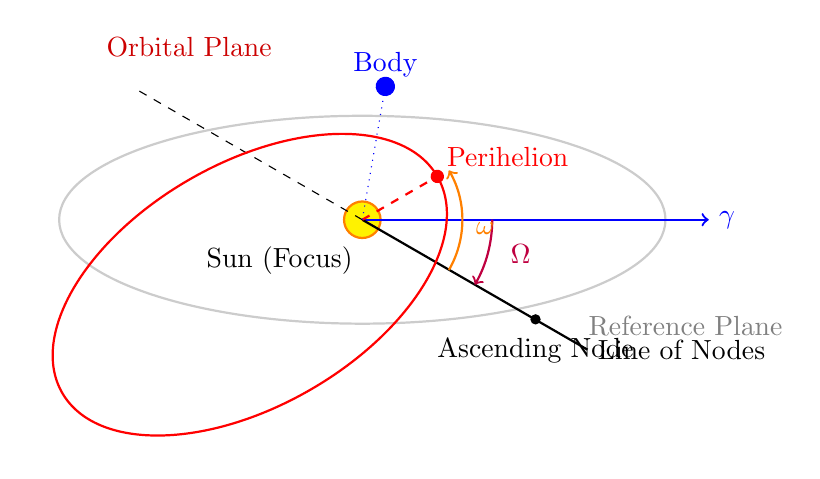
\begin{tikzpicture}[scale=1.1]
    % REFERENCE PLANE (Ecliptic/Equator)
    \draw[thick, gray!40] (0,0) ellipse (3.5cm and 1.2cm);
    \node[gray, below right] at (2.5,-1.0) {Reference Plane};

    % SUN (at Focus/Origin)
    \filldraw[yellow, draw=orange, thick] (0,0) circle (6pt);
    \node[below left] at (0,-0.2) {Sun (Focus)};

    % REFERENCE DIRECTION (Gamma)
    \draw[->, thick, blue] (0,0) -- (4,0) node[right] {$\gamma$};

    % LINE OF NODES
    % Visual intersection roughly at -30 degrees
    \draw[dashed, black] (0,0) -- (-2.6, 1.5); % Descending node side
    \draw[thick, black] (0,0) -- (2.6, -1.5) node[right] {Line of Nodes};
    
    % Ascending Node point
    \filldraw[black] (2.0, -1.15) circle (1.5pt);
    \node[below] at (2.0, -1.25) {Ascending Node};

    % LONGITUDE OF ASCENDING NODE (Omega)
    % Arc from Gamma to Node
    \draw[->, purple, thick] (1.5,0) arc (0:-30:1.5);
    \node[purple, right] at (1.6,-0.4) {$\Omega$};

    % ORBITAL PLANE
    % Rotated so Perihelion is distinct from Node
    % Let's orient perihelion at +30 degrees visual.
    % Ellipse parameters: a=2.5, e=0.6 => c=1.5. Center at (-1.5, 0) relative to axis.
    \begin{scope}[rotate=30]
        % Orbit Path
        \draw[thick, red] (-1.5, 0) ellipse (2.5cm and 1.4cm);
        
        % Perihelion (closest point to focus at 0,0)
        \filldraw[red] (1.0, 0) circle (2pt) node[above right] {Perihelion};
        \draw[thick, red, dashed] (0,0) -- (1.0, 0); % Radius vector to perihelion
        
        % Body Position (True Anomaly nu)
        \filldraw[blue] (1.0, 1.2) circle (3pt) node[above] {Body};
        \draw[dotted, blue] (0,0) -- (1.0, 1.2);
    \end{scope}

    % ARGUMENT OF PERIHELION (omega)
    % Angle from Node (-30 deg) to PeriAxis (+30 deg)
    \draw[->, orange, thick] (1.0, -0.58) arc (-30:30:1.15);
    \node[orange, right] at (1.2, -0.1) {$\omega$};

    % INCLINATION (i)
    % Symbolized by vector relations or just label
    \node[red!80!black] at (-2, 2) {Orbital Plane};
    
\end{tikzpicture}

\caption{Classical Keplerian orbital elements. The orbital plane (red ellipse) is tilted relative to the reference plane. The ascending node is where the orbit crosses the reference plane going northward.}
\label{fig:keplerian_elements}
\end{figure}

\subsection{Orbital Period}

For elliptical orbits, Kepler's Third Law relates period to semi-major axis:
\begin{equation}
    P = 2\pi\sqrt{\frac{a^3}{\mu}}
\end{equation}
where $\mu = GM$ is the gravitational parameter of the central body.

For the Sun:
\begin{equation}
    P[\text{years}] = a[\text{AU}]^{3/2}
\end{equation}

Examples:
\begin{itemize}
    \item Earth: $a = 1$ AU $\Rightarrow P = 1$ year
    \item Mars: $a = 1.524$ AU $\Rightarrow P = 1.88$ years
    \item Ceres: $a = 2.77$ AU $\Rightarrow P = 4.61$ years
\end{itemize}

\subsection{Orbital Energy}

The specific orbital energy (energy per unit mass) is:
\begin{equation}
    \mathcal{E} = -\frac{\mu}{2a}
\end{equation}

Note that $\mathcal{E} < 0$ for elliptical orbits (bound), $\mathcal{E} = 0$ for parabolic, and $\mathcal{E} > 0$ for hyperbolic.

\subsection{Singularities of Keplerian Elements}

Keplerian elements have mathematical singularities:
\begin{itemize}
    \item $\Omega$ undefined for $i = 0^\circ$ (orbit in reference plane)
    \item $\omega$ undefined for $e = 0$ (circular orbit, no perihelion)
    \item Both $\Omega$ and $\omega$ undefined for $i = 0^\circ$ and $e = 0$ simultaneously
\end{itemize}

For near-circular or near-equatorial orbits, numerical errors can grow large. Alternative element sets avoid these issues.

\section{Cartesian State Vector}

The \textbf{Cartesian state vector} specifies position and velocity in a reference frame:
\begin{equation}
    \mathbf{X} = \begin{pmatrix} \mathbf{r} \\ \mathbf{v} \end{pmatrix} = \begin{pmatrix} x \\ y \\ z \\ \dot{x} \\ \dot{y} \\ \dot{z} \end{pmatrix}
\end{equation}

\subsection{Advantages}
\begin{itemize}
    \item No singularities
    \item Simple equations of motion: $\ddot{\mathbf{r}} = -\mu \mathbf{r}/r^3 + \mathbf{a}_{\text{pert}}$
    \item Direct use in numerical integrators
    \item Easy to include perturbations
\end{itemize}

\subsection{Disadvantages}
\begin{itemize}
    \item Less intuitive than Keplerian elements
    \item Difficult to interpret orbital geometry directly
    \item Six tightly coupled variables in integration
\end{itemize}

\subsection{Conversion: Keplerian to Cartesian}

Given Keplerian elements $(a, e, i, \Omega, \omega, M)$ at epoch $t_0$:

\textbf{Step 1}: Solve Kepler's equation for eccentric anomaly $E$:
\begin{equation}
    M = E - e\sin E
\end{equation}
(Requires iterative solution, e.g., Newton-Raphson)

\textbf{Step 2}: Compute true anomaly $\nu$:
\begin{equation}
    \nu = 2\arctan\left(\sqrt{\frac{1+e}{1-e}}\tan\frac{E}{2}\right)
\end{equation}

\textbf{Step 3}: Position and velocity in orbital plane:
\begin{align}
    r &= a(1 - e\cos E) \\
    \mathbf{r}_{\text{orb}} &= r\begin{pmatrix} \cos\nu \\ \sin\nu \\ 0 \end{pmatrix} \\
    \mathbf{v}_{\text{orb}} &= \sqrt{\frac{\mu}{a}}\begin{pmatrix} -\sin E \\ \sqrt{1-e^2}\cos E \\ 0 \end{pmatrix}
\end{align}

\textbf{Step 4}: Rotate to reference frame using rotation matrix:
\begin{equation}
    \mathbf{R}_{3}(-\omega)\mathbf{R}_{1}(-i)\mathbf{R}_{3}(-\Omega)
\end{equation}
where $\mathbf{R}_1(\theta)$ and $\mathbf{R}_3(\theta)$ are rotations about the 1- and 3-axes.

\subsection{Conversion: Cartesian to Keplerian}

Given position $\mathbf{r}$ and velocity $\mathbf{v}$:

\textbf{Step 1}: Compute angular momentum:
\begin{equation}
    \mathbf{h} = \mathbf{r} \times \mathbf{v}
\end{equation}

\textbf{Step 2}: Compute node vector:
\begin{equation}
    \mathbf{n} = \mathbf{\hat{z}} \times \mathbf{h}
\end{equation}

\textbf{Step 3}: Compute eccentricity vector:
\begin{equation}
    \mathbf{e}_{\text{vec}} = \frac{1}{\mu}\left[(\mathbf{v} \times \mathbf{h}) - \mu\frac{\mathbf{r}}{r}\right]
\end{equation}

\textbf{Step 4}: Extract elements:
\begin{align}
    a &= \frac{1}{2/r - v^2/\mu} \\
    e &= |\mathbf{e}_{\text{vec}}| \\
    i &= \arccos\frac{h_z}{|\mathbf{h}|} \\
    \Omega &= \arctan\frac{n_y}{n_x} \\
    \omega &= \arccos\frac{\mathbf{n} \cdot \mathbf{e}_{\text{vec}}}{|\mathbf{n}||\mathbf{e}_{\text{vec}}|} \\
    \nu &= \arccos\frac{\mathbf{e}_{\text{vec}} \cdot \mathbf{r}}{|\mathbf{e}_{\text{vec}}||\mathbf{r}|}
\end{align}

Then $M = E - e\sin E$ where $E = 2\arctan\left(\sqrt{\frac{1-e}{1+e}}\tan\frac{\nu}{2}\right)$.

\section{Equinoctial Elements}

\textbf{Equinoctial elements} avoid singularities at zero inclination and eccentricity. They are particularly useful for asteroids with nearly circular or low-inclination orbits.

\subsection{Definition}

The equinoctial set is:
\begin{align}
    a &= \text{semi-major axis (same as Keplerian)} \\
    h &= e\sin(\omega + \Omega) \\
    k &= e\cos(\omega + \Omega) \\
    p &= \tan(i/2)\sin\Omega \\
    q &= \tan(i/2)\cos\Omega \\
    \lambda &= M + \omega + \Omega \quad \text{(mean longitude)}
\end{align}

\subsection{Conversion to Keplerian}

From equinoctial to Keplerian:
\begin{align}
    e &= \sqrt{h^2 + k^2} \\
    i &= 2\arctan\sqrt{p^2 + q^2} \\
    \Omega &= \arctan\frac{p}{q} \\
    \omega &= \arctan\frac{h}{k} - \Omega \\
    M &= \lambda - \omega - \Omega
\end{align}

\subsection{Advantages}

\begin{itemize}
    \item No singularities for $i \approx 0$ or $e \approx 0$
    \item Smooth evolution near circular/equatorial orbits
    \item Used in JPL's HORIZONS system
    \item Well-suited for numerical orbit propagation
\end{itemize}

\section{Delaunay Elements}

\textbf{Delaunay elements} are a canonical set of action-angle variables used in perturbation theory and Hamiltonian mechanics.

\subsection{Definition}

The Delaunay variables are:
\begin{align}
    L &= \sqrt{\mu a} \quad &\text{(action conjugate to } \ell = M) \\
    G &= L\sqrt{1-e^2} \quad &\text{(action conjugate to } g = \omega) \\
    H &= G\cos i \quad &\text{(action conjugate to } h = \Omega)
\end{align}

The angles are:
\begin{align}
    \ell &= M \quad \text{(mean anomaly)} \\
    g &= \omega \quad \text{(argument of perihelion)} \\
    h &= \Omega \quad \text{(longitude of ascending node)}
\end{align}

\subsection{Properties}

\begin{itemize}
    \item $(L,G,H,\ell,g,h)$ form a canonical coordinate set
    \item Hamiltonian formulation: $\dot{q}_i = \partial H/\partial p_i$, $\dot{p}_i = -\partial H/\partial q_i$
    \item Unperturbed Hamiltonian: $H_0 = -\mu^2/(2L^2)$ (depends only on $L$)
    \item For unperturbed Kepler problem: $L, G, H$ are constants
    \item Useful for secular perturbation theory and resonance analysis
\end{itemize}

\section{AstDyn Implementation}

AstDyn provides conversion functions in the \texttt{OrbitalElements} class:

\begin{lstlisting}[language=C++,caption={Orbital element conversions in AstDyn}]
#include <astdyn/core/OrbitalElements.hpp>
#include <astdyn/core/StateVector.hpp>

using namespace astdyn;

// Keplerian elements
OrbitalElements kep;
kep.a = 2.77;        // AU
kep.e = 0.078;
kep.i = 10.6 * DEG_TO_RAD;  // radians
kep.Omega = 80.3 * DEG_TO_RAD;
kep.omega = 73.1 * DEG_TO_RAD;
kep.M = 15.2 * DEG_TO_RAD;
kep.epoch = 2460000.0;  // JD

// Convert to Cartesian
StateVector sv = kep.to_state_vector();
std::cout << "Position: " << sv.r.transpose() << " AU\n";
std::cout << "Velocity: " << sv.v.transpose() << " AU/day\n";

// Convert back to Keplerian
OrbitalElements kep2 = OrbitalElements::from_state_vector(
    sv.r, sv.v, sv.t
);

// Verify round-trip
std::cout << "Delta a: " << kep2.a - kep.a << " AU\n";
// Output: Delta a: 3.14e-15 AU (machine precision)

// Convert to equinoctial
auto eq = kep.to_equinoctial();
std::cout << "h = " << eq.h << ", k = " << eq.k << "\n";
std::cout << "p = " << eq.p << ", q = " << eq.q << "\n";
\end{lstlisting}

\section{Summary}

Key points about orbital elements:

\begin{enumerate}
    \item Six parameters specify a two-body orbit (6 degrees of freedom)
    \item \textbf{Keplerian elements} $(a,e,i,\Omega,\omega,M)$ are geometrically intuitive
    \item \textbf{Cartesian state} $(\mathbf{r}, \mathbf{v})$ is simple for numerical work
    \item \textbf{Equinoctial elements} avoid singularities at $e=0$ and $i=0$
    \item \textbf{Delaunay elements} are canonical, useful for perturbation theory
    \item Choice of elements depends on application and orbit characteristics
    \item Conversions between element sets are standard operations in AstDyn
\end{enumerate}

Understanding orbital elements is essential for:
\begin{itemize}
    \item Reading and interpreting observational catalogs
    \item Setting up orbit propagation problems
    \item Analyzing orbital dynamics and perturbations
    \item Choosing appropriate numerical methods
\end{itemize}

In the next chapter, we will study the two-body problem in detail—the foundation of orbital mechanics and the basis for all perturbation analyses.
